% Chapter 3

\chapter{A Multi-stage Weibull Hazard Model with Tunnel Application} % Write in your own chapter title
\label{Chapter3}
\lhead{Chapter 3. \emph{Multi-stage Weibull Hazard Model with Tunnel Application}} % Write in your own chapter title to set the page header

\section{General introduction}
\label{31}
Effective management of any infrastructure utilities such as tunnel lighting in highway systems requires comprehensive understanding of the entire operational processes of the utility as well as monitoring of its performance and conditions throughout its operational life. Continuous inspection and monitoring of the system are, however, often technically or financially difficult. Therefore, a need to develop an analytical deterioration forecasting model that can estimate the deterioration speed of either an individual component or the entire infrastructure system has been widely recognized. 

Various studies have attempted incorporation of historical background of infrastructure performance into a deterioration model. For example, \citet{aokia} proposed the Weibull distribution function to estimate the deterioration of lighting facilities in tunnel systems. This expressed the condition state of tunnel lighting facilities in binary terms. However, it is known that the actual deterioration process of most infrastructure systems is better described by plural discrete condition states \cite{shahin05}. In order to overcome this limitation, the Markovian transition probability can be used to express two or more condition states in the deterioration process of infrastructure.

The Markov chain model is a stochastic approach that is widely used to forecast the deterioration speed of an infrastructure system such as a bridge network \cite{madanat95,Guido04,Robelin07,Morcous05}. \citet{toukei} and \citet{kobayashitsuda} further improved the Markov chain model by proposing a handy methodology to estimate the Markovian transition probability. The advantages of these models are that they predict future deterioration according to information from two inspection times and they do not  require extensive historical data.

This chapter proposes a new deterioration forecasting model for infrastructure management, which expresses the deterioration speed in two or more condition states in conjunction with elapsed time,  and follows the Weibull distribution function. To begin with, sections \ref{33} and \ref{34} detail the mathematical formulation of the time-dependent transition probability using the Weibull distribution function and the estimation approach. Section \ref{35} presents an empirical study using actual data from a tunnel lighting system in Japan. Finally, the conclusion summarizes the contributions made by this paper, and points out future research needs.
%%%%
%\section{General Background}
%\label{32}
%\subsection{Outline of Literature Review}
%\label{321}
%In the field of infrastructure management, various models on deterioration forecasting have been widely documented. One major feature of the models is to simulate the deterioratoin process. Beside, the models can be ultilized for setting up the maintenance and repair strategies as well as proposing life cycle cost analysis. Especially, under requirement of infrastructure management at network level, these objectives is particular imperative \citep{aokia,kobayashitsuda}.
%
%Many past researches had paid much attention to the physical mechanism of deterioration  of structures \cite{mishalani95,steven}.However, these researches remain in rudiment stage of development as not clearly specifying the statistical estimation method. And thus, several problems from the estimation results can be seen as the limitations. Moreover, a great numbers of inspection data is generally required to ensure the accuracy of the models.
%
%In recent decades, studies toward statistical application have been extensively recorded   \cite{lancaster90,gouri}. For instance, \citet{shin} proposed to employ Weibull deterioration hazard model to forecast the crack starting time on pavement structures. In similar approach, \citet{aokia} empirically verified the effectiveness of applying Weibull distribution function to forecast the deterioration of tunnel lighting facilities. However, as earlier mentioned, these models portrayed the deterioration progress only by using binary condition state, and thus, does not totally reflect the actual plural condition states applied in infrastructure management. 
%
%Efforts in tackling the emerging problems had been proposed. A typical example is multi-stage model developed by \citet{lancaster90} for the behavior of labor transition. In which, he described a rational approach to estimate the transition probability from multiple condition states. The mechanism in multi-stage model is that the condition state changes from one state to other states only in one-step. This boundary limits its application into infrastructure management since the condition state transitions are often observed in more than one-steps changes. In an effort to tackle this limitation, \citet{kobayashitsuda} described the vertical transitive relation between condition states, and proposed a method to estimate Markov transition probability according to multi-stage hazard model for bridge management.

%Markov hazard model proposed by \citet{kobayashitsuda} has wide applicability into many fields. However, the Markov transition probability has the characteristic that the deterioration process does not depend on the past deterioration history. Additionally, there is no concrete guarantee that the deterioration process genuinely satisfies the Markov characters. Especially, in the case when the total operation duration of infrastructure is taken into estimation. This appealing has generated a motivation for development of this paper, which considers either multi-state transition between condition states and historical operation time.
%%%%
\section{Formulation of the Model}
\label{33}
\subsection{Deterioration State Probability}
\label{331}
We denote $s$ as an arbitrary elapsed time counted from the initial time $\tau_0$. The state variable $h(s)$ expresses the actual condition state corresponding to time $\tau = \tau_0 + s$. The deterioration process is described by using conditional probability, which describes condition state $h(s) = i$ as occuring at time $s$ dependent on the given condition state at $\tau_0$ (hereafter  referred to deterioration state probability):
\begin{eqnarray}
&& \mbox{Prob}[h(s)=i|h(0)=1]=\pi_{i}(s).\label{pro3}
\end{eqnarray}
If the deterioration state probability $\pi_{i}$ is defined in the range of condition state $i (i=1,...,I)$, then a time dependence deterioration state probability vector can be further expressed as
\begin{eqnarray}
&& {\bf \Pi}(s)=\left(
\begin{array}{c}
\pi_{1}(s) \\
\vdots \\
\pi_{I}(s)
\end{array}
\right).
\end{eqnarray}
The deterioration state probability in equation (\ref{pro3}) represents the probability of each condition state $i$ being observed at time $\tau = \tau_0 + s$. In other words, it expresses the  probability of state occurrence in the elapsed time $s$ from the initial time. The summation $\sum_{i=1}^{I}\pi_{i}(s) = 1 $ is justified by the definition of deterioration state probability.
\subsection{Deterioration State Probability from Initial Time}
\label{332}
We assume the opening of an infrastructure facility at time $\tau_0$ with condition state $1$ (Fig. \ref{fig26}). At time $\tau$, the observed condition state is $i$. On the horizontal time axis, condition states of the infrastructure facility can be displayed with respect to arbitrary time from $\tau_0$ to $\tau$. The probability of the event that condition state $1$ changes to condition state $i$ can be represented by state probability $\pi_{i} (s)$ (where, $s = \tau - \tau_0$):
\subsubsection{a) $i=1$ }
\label{3321}
Condition state remains as $1$ until time $\tau$. The deterioration state probability  $\pi_{1}(s)$ is exactly equal to the survival probability expressed in equation (\ref{prop-bFla}):
\begin{eqnarray}
&& \pi_{1}(s)=\tilde{F}_1(s) = \exp (-\theta_1 s^{\alpha_{1}}). \label{ii1}
\end{eqnarray}
\subsubsection{b) $i=2$ }
\label{3322}
In the case when condition state $i=2$ is observed at time $\tau$, the condition state changes from $1$ to $2$ at time $\tau_1 \in [\tau_0, \tau]$. The probability density that the life span of condition state $1$ becomes $\zeta_1=\tau_1-\tau_0$ can be expressed as $f_1(\zeta_1)$ by using the Weibull function. $\zeta_1~(\geq 0)$ is a random variable, which owns its value in the following range:
\begin{eqnarray}
&& 0\leq \zeta_1 < s. \label{hanni}
\end{eqnarray}
State probability $\pi_{2} (s)$ with condition state $i=2$ being observed at time $\tau$ is shown in the next equation: 
\begin{eqnarray}
&& \pi_{2}(s) =\int_{0}^{s} f_{1}(\zeta_1)\tilde{F}(s-\zeta_1)d\zeta_1. \label{i2}
\end{eqnarray}
\subsubsection{c) $3\leq i<I$}
\label{3323}
For a general case, as condition state at time $\tau$ can take value between $3\leq i<I$, the event of changes in condition state will occur at respective times $\tau_1,\cdots,\tau_{i-1}~(\tau_0\leq \tau_1 \leq \cdots \leq \tau_{i-1}< \tau)$. The following steps describe the mechanism of these changes. At first, condition state $1$  remains in a duration from time $\tau_0$ to time $\tau_0+\zeta_{1}\in [\tau_{0},\tau]$, as illustrated in Fig. \ref{fig31}. Secondly, at time $\tau_1$, condition state changes from $1$ to $2$. Thirdly, condition state $2$ remains in a duration from time $\tau_1$ until time $\tau_2=\tau_{1}+\zeta_{2}\in [\tau_1,\tau]$, before turning into condition state $3$ exactly at time $\tau_2$. Fourthly, after undergoing similar processes, condition state advances to $i$ at time $\tau_{i-1}=\tau_{i-2}+\zeta_{i-1}\in [\tau_{i-2},\tau]$, and remains at condition state $i$ until time $\tau$. To simulate the occurrence of these events, we use the probability density $q_{i} (\zeta_1,,\cdots,\zeta_{i-1})$ in the entire duration $s=\tau-\tau_{0}$:
%%
\begin{eqnarray}
&& \hspace{-5mm} q_{i}(\bar{\zeta}_1,\cdots,\bar{\zeta}_{i-1})
 = \prod_{m=1}^{i-1} f_{m}(\bar{\zeta}_m) \tilde{F}_{i}(s-\sum_{m=1}^{i-1}\bar{\zeta}_m).
\end{eqnarray}
Random variable $\zeta_m~(\geq 0)$ takes its value in the range to satisfy
\begin{eqnarray}
&& 0\leq \zeta_1+\zeta_{2}+\cdots+\zeta_{i-1} < s. \label{hani}
\end{eqnarray}
Therefore, the state probability  $\pi_{i} (s)$, which represents observed condition state $i~(i=3,\cdots,I-1)$ at time $\tau=\tau_0+s$, can be expressed as follows:
\begin{eqnarray}
&& \pi_{i}(s)=\int_{0}^{s}\int_0^{s-\zeta_{1}} \cdots
\int_{0}^{s-\sum_{m=1}^{i-2}\zeta_{m}}
 q_{i}(\zeta_1,\cdots,\zeta_{i-1}) d\zeta_1\cdots d\zeta_{i-1}. \label{dousyutu1}
\end{eqnarray}
\subsubsection{d) $i=I$ }
\label{3324}
Condition state $I$ is absorbing state, which refers to the worst deterioration. At the time when $I$ has been reached, if no repair occurs, the state $I$ will remain forever. From the definition of the deterioration state probability, the probability of observing absorbing state $I$ is shown in the following equation:
\begin{eqnarray}
&& \pi_I(s)=1-\sum_{m=1}^{I-1}\pi_m(s).\label{oo}
\end{eqnarray}

\begin{figure}[t]
\begin{center}
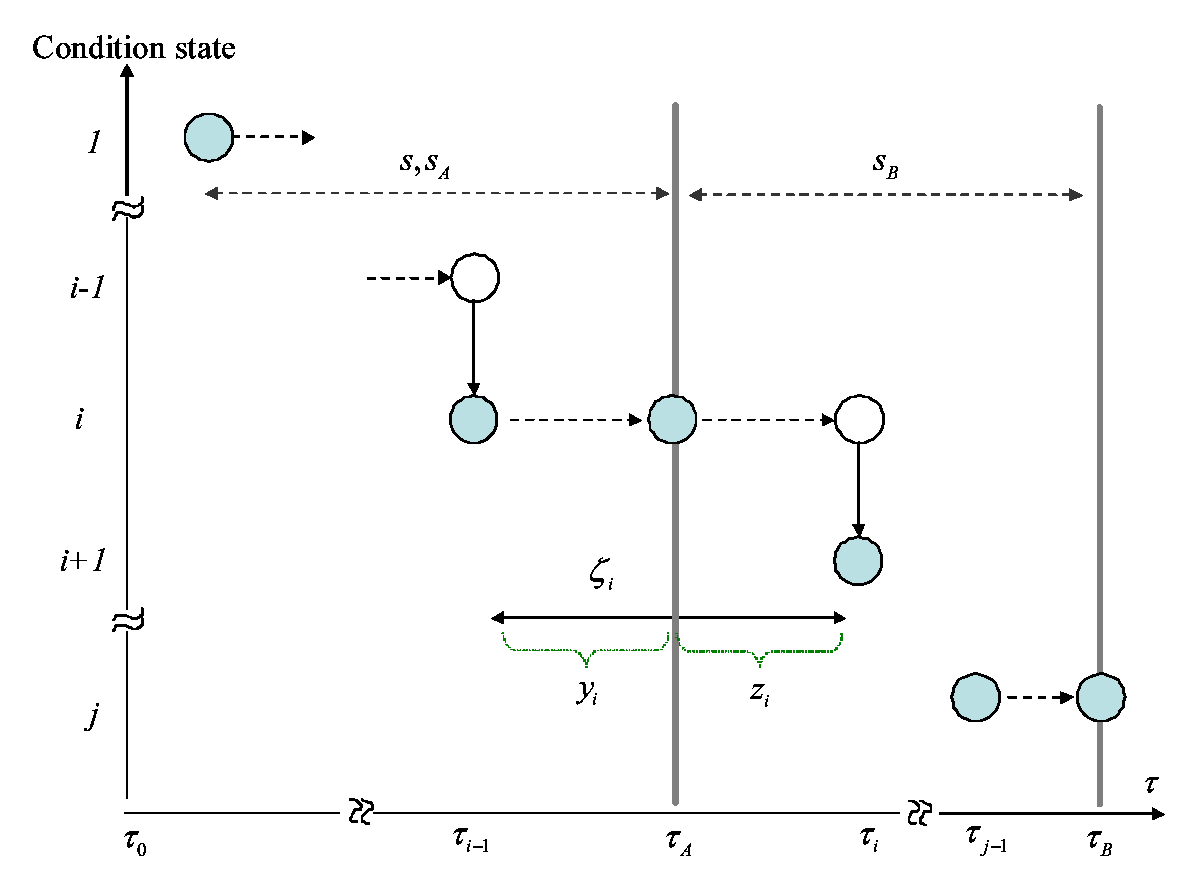
\includegraphics[scale=0.5]{fig31} 
\end{center}
\footnotesize Note) In the figure, the initial time is $\tau_0$. Condition state $i$ is observed at time $\tau_A$. For two inspection times $\tau_A$ and $\tau_B$, we represent $s_A=\tau_A-\tau_0$, $s_B=\tau_B-\tau_A$ as elapsed time. The time length $y_i$ is measured from time $\tau_{i-1}$ to time $\tau_A$, and $z_i$ is measured from time $\tau_A$ to time $\tau_i$. The total life span (survival time) of condition $i$ is expressed as $\zeta_i=y_i+z_i$.
\caption{Deterioration from Initial Time and Observation of Condition State.}
\label{fig31} 
\end{figure}%[t]
%%
\subsection{Simultaneous Occurrence Probability of Condition State at Two or More Times}
\label{333}
We assume that there are two inspection times $\tau_A$ and $\tau_B$, at which the condition states $i$ and $j$ $(i\leq j;j=1,\dots,I-1)$ are observed respectively. $\tau_{0}$ is the initial time of the deterioration process as shown in Fig. \ref{fig31}. The transition pattern of condition states occurs in the following steps. Firstly, at time $\tau_{i-1}$, condition state $i-1$ changes into condition state $i$. However, condition state $i$ can be revealed only at inspection time $\tau_A$. The duration of this event can therefore be defined as $\tau_A=\tau_{i-1}+y_i$. Secondly, at time $\tau_i=\tau_A+z_i$, the condition state advances from $i$ to $i+1$. Thirdly, condition state $i+1$ will rise to $j-1$ at time $\tau_{j-1}$. Finally, after $\tau_{j-1}$, the condition state will reach $j$ and remain in condition state $j$ until inspection time $\tau_B$. 

In Fig. \ref{fig31}, we define durations $s_A=\tau_A-\tau_0$ and $s_B=\tau_B-\tau_A$. It should be recognized from Fig. \ref{fig31} that condition state $i-1$ changes into condition state $i$ at time $\tau_{i-1}=\tau_A-y_i$. In other words, condition state $i$ is revealed at inspection time $\tau_A$;  however, it has already existed over the duration $y_i$. In addition, we define $\zeta_i$ as the life span of condition state $i$. If condition state $j$ observed at inspection $\tau_B$ is considered, the probability for this event to happen is thus dependent on the information concerning condition state $i$. Thus, by the law of conditional probability, the following conditional probability density function is defined:
\begin{eqnarray}
&& \hspace{-5mm} g_{ij}(s_B,\bar{z_i},\bar{\zeta}_{i+1},\cdots,\bar{\zeta}_{j-1}|\bar{y}_i)=\frac{f_i(\bar{y}_i+\bar{z}_i)}{\tilde{F}_i(\bar{y}_i)} \nonumber \\
&& \prod_{m=i+1}^{j-1}f_m(\bar{\zeta}_m) \tilde{F}_j(s_B-\bar{z}_i-\sum_{m=i+1}^{j-1}\bar{\zeta}_m).
\label{pt12}
\end{eqnarray}
In equation (\ref{pt12}), $y_i$ and $z_i$ are the durations measured from time $\tau_{i-1}$ to time $\tau_A$ and from time $\tau_A$ to time $\tau_i$ respectively, as shown in Fig. \ref{fig31}. The life span of condition state $i$ is defined by means of variable $\zeta_i=y_i+z_i$. Variables $z_i~(\geq 0),\zeta_{i+1}~(\geq 0),$ $\cdots,\zeta_{j-1}~(\geq 0)$ are random variables with their values to satisfy the following equation:
\begin{eqnarray}
&& 0\leq z_i+\sum_{m=i+1}^{j-1} \zeta_m < s_B.
\end{eqnarray}
Given the elapsed time $y_i$ and condition state $i$ observed at inspection time $\tau_A$, we define the conditional probability $\kappa_{ij} (s_B|y_i)$, to which condition state $j$ is observed at inspection time $\tau_B=\tau_A+s_B$:
\begin{eqnarray}
\hspace{-3mm} \kappa_{ij}(s_B|\bar{y}_i)=\int_0^{s_B}\int_0^{s_B-z_i} \cdots \int_{0}^{s_B-z_i-\sum_{m=i+1}^{j-2}\zeta_m} \nonumber \\
\hspace{2mm} g_{ij}(s_B,z_i,\zeta_{i+1},\cdots,\zeta_{j-1}|\bar{y}_i)dz_i d\zeta_{i+1}\cdots d\zeta_{j-1}.
\end{eqnarray}
Condition state $i$ can appear at any arbitrary time from the initial time to inspection time $\tau_A$. The duration $y_i$ therefore has a range in the domain $0\leq y_i\leq s_A$. Eventually, we can define the probability density $\eta_{i} (s_A,y_i)$, which describes the probabilistic relation of condition state $i$ occurring at time $\tau_{i-1} = \tau_A-y_i$:
\begin{eqnarray}
&& \eta_{i}(s_A,y_i)=\Bigg\{\int_0^{s_A-y_i} \int_0^{s_A-y_i-\zeta_1}\cdots \nonumber \\
&& \hspace{9mm} \int_0^{s_A-y_i-\sum_{m^\prime=1}^{i-3}\zeta_{m^\prime}}
\prod_{m^\prime=1}^{i-1} f_{m^\prime}(\zeta_{m^\prime}) 
 d\zeta_1\cdots d\zeta_{i-2}\Bigg\} \tilde{F}_i(y_i), \\
&& \zeta_{i-1}=s_A-y_i-\sum_{m^\prime=1}^{i-2}\zeta_{m^\prime}. \nonumber
\end{eqnarray}
As a sequel, we are able to define the explicit form for transition probability $\pi_{ij}(s_A,s_B)$, which expresses the conditional probability for condition state $i$ being observed at $\tau_A$ and condition state $j$ being observed at $\tau_B=\tau_0+s_A+s_B$:
\begin{eqnarray}
&& \hspace{-18mm}\pi_{ij}(s_A,s_B)=\mbox{Prob}[h(s_A)=i,h(s_A+s_B)=j] 
 =\int_{0}^{s_A}\eta_{i}(s_A,y_i)\kappa_{ij}(s_B|y_i)dy_i. \label{dousyutu3} 
\end{eqnarray}
The probability that condition state $I$ is observed at inspection time $\tau_A$ can be seen in  equation (\ref{oo}). If at inspection $\tau_B$, condition state $I$ is revealed, we can define the following transition probability:
\begin{eqnarray}
&& \pi_{iI}(s_A,s_B)=\pi_i(s_A)-\sum_{j=i}^{I-1}\pi_{ij}(s_A,s_B).\label{dousyutu4}
\end{eqnarray}
\subsection{Management Indicators for Infrastructure Management}
\label{334}
The life expectancy of condition state $i$ is an important indicator for infrastructure management. Life expectancy is viewed as duration, in which condition state $i$ remains until entering condition state $i+1$. In other words, life expectancy of condition state $i$ is the remaining duration counted from initial time until time $\tau_i$, at which, condition state $i$ changes to condition state $i+1$. Probabilistically, life expectancy of condition state $i$ can be expressed by means of the survival probability function $\tilde{F}_i(y_i)$ \cite{lancaster90}:
\begin{eqnarray}
&& RMD(i)= \int^{\infty}_{0}\tilde{F}_i(y_i)dy_i. \label{173}
\end{eqnarray}
The abbreviation $RMD$ stands for ``Remaining Duration''. Based on equation (\ref{prop-bFla}), we have the following equation:
\begin{eqnarray}
&& RMD(i)= \int^{\infty}_{0}\exp (-\theta_i y_i^{\alpha_i}) dy_i. \label{rating3}
\end{eqnarray}
Management indicator $RMD(i)$ is estimated based on the assumption that at time $\tau_{i-1}$ condition state changes from $i-1$ to $i$, as shown in Fig. \ref{fig31}. This calculation seems to have the  limitation that it does not capture the historical duration measured from initial time. Thus, it is necessary to define the life expectancy of condition state $i$ based on the initial time. We denote $RL(i)$, standing for ``Remaining Life'', as a management indicator, which indicates the duration of condition state $i$ counted from initial time. As can be seen from Fig. \ref{fig31}, $RL(i)$ is actually measured from time $\tau_0$ to time $\tau_i$. Given the total duration $s$ for condition state $i$ to  remain until reaching condition state $i+1$, we can define the probability density $\rho_{i}(s)$ for condition state $i$ ending its service life at time $\tau=\tau_0+s$:
\vspace{1mm}
\begin{eqnarray}
\rho_{i}(s)= \int_0^s \int_0^{s-\zeta_1} \cdots \int_{0}^{s-\sum_{m=1}^{i-2} \zeta_m} 
 \prod_{m=1}^{i-1} f_{m}(\zeta_m) f_i(s-\sum_{m=1}^{i-1} \zeta_m)d\zeta_1\cdots d\zeta_{i-1}.
\end{eqnarray}
$RL(i)$ is the expected period until the ending of condition state $i$ counted from initial time, and thus can be further defined:
\begin{eqnarray}
&& RL(i)=\int_{0}^\infty s \rho_i(s) ds. \label{r1}
\end{eqnarray}
It is noted that $RMD$ and $RL$ are fundamentally estimated based on two different assumptions of starting time. Thus, there exists a high possibility that the estimation results of these two management indicators are different. In addition to management indicators $RMD(i)$ and $RL(i)$, there is a need to estimate the life expectancy of condition state $j$ as well. As a matter of fact, the event condition state $j$ appears conditionally dependent on condition state $i$, which seems to be observed at inspection time $\tau_A$. By the law of conditional probability, we can define the conditional probability density $\nu_{j}(s|h(s_A)=i)$, at which condition state will disappear given the visual observed condition state $i$ at time $\tau_A=\tau_0+s_A$ and the elapsed duration time $s$:
\begin{eqnarray}
&& \hspace{-2mm} \nu_{j}(s|h(s_A)=i) = \frac{M*N}{\pi_i(s_A)}, \label{eq30}
\end{eqnarray}
where,
\begin{eqnarray}
&& M = \int_{0}^{s_A}
\int_0^{s_A-y_i} \int_0^{s_A-y_i-\zeta_1}\cdots \int_0^{s_A-y_i-\sum_{m^\prime=1}^{i-3}\zeta_{m^\prime}}f_i(y_i+z_i)\cdot \nonumber\\
&& \hspace{80mm}\prod_{m^\prime=1}^{i-1} f_{m^\prime}(\zeta_{m^\prime})dy_i d\zeta_1\cdots d\zeta_{i-2}dz_i, \nonumber \\
&& N = \int_0^{s}\int_0^{s-z_i} \cdots \int_{0}^{s-z_i-\sum_{m=i+1}^{j-2}\zeta_m }\prod_{m=i+1}^{j-1}f_m(\zeta_m)  \nonumber \\
&& \hspace{75mm}f_j(s-z_i-\sum_{m=i+1}^{j-1} \zeta_m)d\zeta_{i+1}\cdots  d\zeta_{j-1}, \nonumber \\
&& (i\leq j; j=1,\cdots,I-1) \hspace{3mm} \text{and} \hspace{3mm} \zeta_{i-1}=s_A-y_i-\sum_{m^\prime=1}^{i-2}\zeta_{m^\prime}. \nonumber
\end{eqnarray}
The denominator of equation (\ref{eq30}) refers to deterioration state probability for condition state $i$, which remains until time $s_A$. In the numberator, $M$ represents the event that condition state $i$ remains until increment time $z_i$, and  $N$ represents the event that condition state $i$ changes to $j$ at elapsed time $\zeta_{j-1}$ and stays up to duration $s$. Eventually, we define the life expectancy of condition state $j$ ($j \geq i$) as $RL_{j}(h(s_A)=i)$, which conditionally depends on condition state $i$ with duration $s_A$:
%%%%%%%%%55
\begin{eqnarray}
&&\hspace{-3mm}  RL_{j}(h(s_A)=i)=\int_{0}^{\infty} s \nu_j(s|h(s_A)=i)ds,
\label{r2}\\
&& (i\leq j; i,j=1,\cdots,I-1). \nonumber
\end{eqnarray}
%%%
\section{Estimation Method}
\label{34}
\subsection{Content of Data from Visual Inspection}
\label{341}
Suppose visual inspection data on the same kind of $K$ infrastructure components is available. An inspection sample $k~(k=1,\cdots,K)$ describes two visual inspection times carried out at initial time $\bar{\tau}_0^k$ and $\bar{\tau}_A^k$ with the concerning condition state $h(\bar{s}^k)$. The symbol $\lfloor\bar{\text{    }}\rceil$ indicates an actual measurement. $\bar{s} ^k=\bar{\tau} _ A^k-\bar{\tau} _ 0^k$ is the duration between two inspection times. In addition, a dummy variable $\bar{\mbox{\boldmath$\delta$}}^k=\{\bar{\delta}_{i}^k~(i=1,\cdots,I)\}$ based on the deterioration progress patterns between two inspection times is defined as
\begin{eqnarray}
&& \bar{\delta}_{i}^k=\left\{
\begin{array}{ll}
1 & h(\bar{s}^k)= i\\
0 & \text{Otherwise}
\end{array}.
\right.
\end{eqnarray}
Furthermore, in order to describe the information in sample $k$, we use characteristic vector  $\bar{\mbox{\boldmath$x$}}^k=(\bar{x}_1^k,\cdots,\bar{x}_N^k)$ and elapsed duration $\bar{s}^k$.  $\bar{x}_n^k~(n=1,\cdots,N)$ represents the value of a characteristic variable $n$ visually observed in the sample $k$. Thus, the information contained in inspection sample $k$ can be rearranged as  $\bar{\xi^k}=(\bar{\mbox{\boldmath$\delta$}}^k,\bar{s}^k,\bar{\mbox{\boldmath$x$}}^k)$. As a result, we can further express the Weibull hazard function for sample $k$ as
%%
%%
\begin{eqnarray}
&& \lambda_i^k(y_i)=\theta_i^k \alpha_{i} y_i^{\alpha_{i}-1} ~(i=1,\cdots,I-1). \label{pt26}
\end{eqnarray}
It is noted that the hazard function is not defined for condition state $I$ since $I$ is absorbing state and $\mathop{\lim}\limits_{s\to\infty}\pi_I(s) = 1$. As a matter of course, the value of hazard rate $\theta_i^k~(i=1,\cdots,I-1;k=1,\cdots,K)$ changes according to the property of characteristic vectors of sample $k$. The dependency of hazard rate on characteristic vector $\bar{\mbox{\boldmath$x$}}^k$ can be formulated by means of functional relationship as
\begin{eqnarray}
&&
\theta_i^k=\bar{\mbox{\boldmath$x$}}^k\mbox{\boldmath$\beta$}_i^\prime\label{hazard13}
\end{eqnarray}
where $\mbox{\boldmath$\beta$}_i=(\beta_{i1},\cdots,\beta_{iN})$ is a row vector of unknown parameter $\beta_{in}~(n=1,\cdots,N)$, and the symbol $\prime$ indicates that the vector is transposed. The functional relationship between hazard rate and characteristic variable can be changed according to  preferences in estimation. This issue can be further viewed in the relationship assumption in our empirical study.

Later in this section, the methodology to estimate the transition probability will be presented. At first, based on the Weibull hazard function $\lambda_i^k(y_i)$ with collected sample information $\bar{\xi^k}~(k=1,\cdots,K)$, the likelihood function for transition probability is defined. Based on the maximum likelihood estimation approach, we can obtain the values for unknown parameters in equation (\ref{hazard13}) and further for the parameterized values of the Weibull hazard function. Secondly, the estimation method is proposed for the transition probability when there are two or more than two inspection data. Finally, we explain the necessity of estimating the expected deterioration probability as a representative value when there is a large pool of sampling data.
%%%%%%
\subsection{Estimate of Weibull Hazard Function}
\label{342}
As earlier mentioned, data concerning inspection sample $k$ can be rearranged as $\bar{\xi^k}=(\bar{\mbox{\boldmath$\delta$}}^k,\bar{s}^k,\bar{\mbox{\boldmath$x$}}^k)$. The application of the Weibull hazard function in estimating the deterioration state probability is discussed in equations  (\ref{ii1}),(\ref{i2}),(\ref{dousyutu1}),(\ref{oo}). Applying the characteristic vector $\bar{\mbox{\boldmath$x$}}^k$ of infrastructure component, we can calculate the hazard rate expressed in equation (\ref{hazard13}). Moreover, the deterioration state probability depends on the duration of operation $\bar{s}^k$ after the opening time of the infrastructure. Therefore, in order to express clearly this characteristic, the deterioration state probability $\pi_{i}(\bar{s}^k)$ can be defined as a function of measured visual inspection data $(\bar{s}^k,\bar{\mbox{\boldmath$x$}}^k)$ and unknown parameter vector $\mbox{\boldmath$\gamma$}=\{\mbox{\boldmath$\alpha$},\mbox{\boldmath$\beta$}_i~(i=1,\cdots,I-1)\}$. $\mbox{\boldmath$\alpha$}=(\alpha_{1},\cdots,\alpha_{I-1})$ is a row vector of unknown parameter $\alpha_{i}~(i=1,\cdots,I-1)$. 

If the deterioration progress of the infrastructure components in  $K$ samples are assumed to be mutually independent, the log-likelihood function expressing the simultaneous probability density of the deterioration transition pattern for all inspection samples is  
\begin{eqnarray}
&& \hspace{-10mm} \ln[{\cal L}(\mbox{\boldmath$\gamma$})] = \ln
\left[\prod_{i=1}^{I} \prod_{k=1}^{K}
\left\{\pi_{i}(\bar{s}^k,\bar{\mbox{\boldmath$x$}}^k:\mbox{\boldmath$\gamma$})\right\}^{\bar{\delta}_{i}^k}\right]
%\nonumber \\
 =\sum_{i=1}^I \sum_{k=1}^{K} \bar{\delta}_{i}^k
\ln\left[
\pi_{i}(\bar{s}^k,\bar{\mbox{\boldmath$x$}}^k:\mbox{\boldmath$\gamma$})\right],
\label{logbF3}
\end{eqnarray}
where $\bar{\mbox{\boldmath$\delta$}}^k$, $\bar{s}^k$, $\bar{\mbox{\boldmath$x$}}^k$ are all determined through inspection and $\mbox{\boldmath$\gamma$}$ is a parameter to be estimated \cite{tobin,amemi}. Estimation of parameter  $\mbox{\boldmath$\gamma$}$, given an amount of $\hat{\mbox{\boldmath$\gamma$}}=(\hat{\gamma}_{10},\cdots,\hat{\gamma}_{I-1N})$, can be obtained by solving the optimality conditions
\begin{eqnarray}
&& \frac{ \partial \ln[{\cal L}(\hat{\mbox{\boldmath$\gamma$}})] }{\partial
\gamma_{in}}=0, \quad ~(i=1,\cdots,I-1;n=0,1,\cdots,N), \label{saiteki3}
\end{eqnarray}
that result from maximizing the log-likelihood function (\ref{logbF3}). The optimal values $\hat{\alpha}_i=\hat{\gamma}_{i0}$ and $\hat{\mbox{\boldmath$\beta$}}_i=(\hat{\gamma}_{i1},\cdots,\hat{\gamma}_{iN})$ are then estimated by applying a numerical iterative procedure such as the Newton method for the $(I-1)\times (N+1)$ order nonlinear simultaneous equations \cite{tuma}. Moreover, estimator for the asymptotical covariance matrix of the parameters ($\hat{\mbox{\boldmath$\Sigma$}}(\hat{\mbox{\boldmath$\gamma$}})$) is given by
\begin{eqnarray}
&& \hat{\mbox{\boldmath$\Sigma$}}( \hat{\mbox{\boldmath$\gamma$}})
= \left[ \frac{ \partial^2\ln\{ {\cal L}( \hat{\mbox{\boldmath$\gamma$}})\}
}{\partial \mbox{\boldmath$\gamma$} \partial \mbox{\boldmath$\gamma$}'}
\right]^{-1}.
\end{eqnarray}
The $(I-1)(N+1)\times (I-1)(N+1)$ order invert matrix of the right-hand side of the above equation, composed of the element $\partial^2\ln\{{\cal L}(\hat{\mbox{\boldmath$\gamma$}})\}/\partial \gamma_{in} \partial \gamma_{i^\prime n^\prime}$ results in the invert matrix of the Fisher information matrix \cite{greene}. In the above-mentioned calculation process, it might not be necessary directly to estimate the deterioration state probability $\pi_i(s)$ from the log-likelihood function of equation (\ref{logbF3}). The deterioration state probability can be estimated from multiple integration of equation (\ref{dousyutu1}). Suffice it to say that the accuracy of estimation for  $\hat{\mbox{\boldmath$\gamma$}}$ depends on the accuracy in calculating the multiple integration. Considering this challenge, in this research we employ double integration, suggested by \citet{steven98}, to improve the accuracy of multiple integral calculation.
%%%%%%%%%
\subsection{Estimation Method for the Case of Having Data from Two or More Visual Inspections}
\label{343}
In general management practice, the database is composed only of data from two inspection times. However, future monitoring activities may be expanded so as to provide the advantage of data for more than two inspection times. Therefore, besides the estimation methodology for two inspection times as earlier discussed, it is necessary to develop a method to take multi-inspection times into account.

For sample $k$, we assume the condition states $h(\bar{s}_A^k)$ and $h(\bar{s}_A^k+\bar{s}_B^k)$ are respectively observed at inspection times $\bar{\tau}_A^k$ and $\bar{\tau}_B^k$. $\bar{\tau}_0^k$ is defined as initial time. Thus, two durations of operation according to two inspection times are further defined as $\bar{s}_A^k=\bar{\tau}_A^k-\bar{\tau}_0^k$ and $\bar{s}_B^k=\bar{\tau}_B^k-\bar{\tau}_A^k$. Additionally, a dummy variable $\mbox{\boldmath$\bar{\Delta}$}^k=\{ \bar{\delta}_{ij}^k~(i=1,\cdots,I-1, j=1,\cdots,I)\}$ is determined based on the transition pattern observed from inspections:
%
\begin{eqnarray}
&& \bar{\delta}_{ij}^k=\left\{
\begin{array}{ll}
1 & h(\bar{s}_A^k)=i,h(\bar{s}_{A}^k+\bar{s}_B^k)= j\\
0 & Otherwise
\end{array}.
\right.
\end{eqnarray}
The information of inspection sample $k$ can be rearranged as $\Xi^k=(\bar{\mbox{\boldmath$\Delta$}}^k,\bar{\mbox{\boldmath$s$}}^k,\bar{\mbox{\boldmath$x$}}^k)$. Since the duration $\bar{\mbox{\boldmath$s$}}^k=(\bar{s}_A^k,\bar{s}_B^k)$ is observable, the deterioration state probability can be estimated according to equations (\ref{dousyutu3}) and (\ref{dousyutu4}). Precisely, the transition probability $\pi_{ij}(\bar{s}_A^k,\bar{s}_B^k)$ can be expressed by means of the function of $\pi_{ij}(\bar{\mbox{\boldmath$s$}}^k,\bar{\mbox{\boldmath$x$}}^k:\mbox{\boldmath$\gamma$})$, in which  the data $(\bar{\mbox{\boldmath$s$}}^k,\bar{\mbox{\boldmath$x$}}^k)$ are available from visual inspections, thus making unknown parameter $\mbox{\boldmath$\gamma$}$ the only target of estimation. The description of unknown parameter $\mbox{\boldmath$\gamma$}=\{\mbox{\boldmath$\alpha$},\mbox{\boldmath$\beta$}_i~(i=1,\cdots,I-1)\}$ is similar to that explained earlier in this section.

In a similar approach to equation (\ref{logbF}), we define the log-likelihood function for transition probability as follows:
\begin{eqnarray}
&& \hspace{-3mm} \ln[{\cal L}(\mbox{\boldmath$\gamma$})] = \ln
\left[\prod_{i=1}^{I-1}\prod_{j=i}^{I} \prod_{k=1}^{K}
\left\{\pi_{ij}(\bar{\mbox{\boldmath$s$}}^k,\bar{\mbox{\boldmath$x$}}^k:\mbox{\boldmath$\gamma$})\right\}^{\bar{\delta}_{ij}^k}\right]
\nonumber \\
&& \hspace{5mm} = \sum_{i=1}^{I-1} \sum_{j=i}^I \sum_{k=1}^{K}\bar{\delta}_{ij}^k
\ln\left[
\pi_{ij}(\bar{\mbox{\boldmath$s$}}^k,\bar{\mbox{\boldmath$x$}}^k:\mbox{\boldmath$\gamma$})\right].
\label{lsogbF}
\end{eqnarray}
By applying the maximum likelihood estimation approach, we can obtain the value for unknown parameter $\hat{\mbox{\boldmath$\gamma$}}$. We will omit a detailed explanation, since this is similar to a reference mentioned earlier in this section. Nevertheless, it is worth emphasizing that the case when $i=I$ is not embedded in the degree of equation (\ref{lsogbF}) since $I$ is the absorbing state.
%%%
\subsection{Expected Deterioration State Probability}
\label{344}
The research methodology for deterioration estimation can be applied to every individual infrastructure component. However, in practice, when the deterioration pattern of a large amount of sampling data is considered, it is more convenient to estimate the expected deterioration state probability rather than to focus on that of individual components. 

With regard to the relationship between the hazard rate $\theta_i^k~(k=1,\cdots,K)$ of sample $k$ and the characteristic variable $x$, it is understandable to express the distribution function of characteristic variable as $\Gamma(\mbox{\boldmath$x$})$. Thus, statistically, the expected value of the hazard rate $E [\theta_i]$ can be defined by means of the distribution function of characteristic variable $x$:
\begin{eqnarray}
&& E[\theta_i]=\int_{\Theta}\mbox{\boldmath$x$}\mbox{\boldmath$\beta$}_i^\prime d\Gamma(\mbox{\boldmath$x$}),\label{oiu3}
\end{eqnarray}
where $\Theta$ refers to the entire sample population. After averaging the value of the hazard rate, we can again define the Weibull hazard function as
\begin{eqnarray}
&& \overline{\lambda}_i(y_i)=E[\theta_i] \alpha_{i} y_i^{\alpha_{i}-1}. \label{hazardg}
\end{eqnarray}
Eventually, after the expected hazard rate is estimated from equation (\ref{hazardg}), the expected deterioration state probability (equations (\ref{ii1}), (\ref{i2}), (\ref{dousyutu1}) and  (\ref{oo})) and the life expectancy of condition states (equations (\ref{r1}) and (\ref{r2})) can be obtained. 
\section{Empirical Study}
\label{35}
\subsection{Overview of Empirical Study}
\label{351}
In this section, we present an empirical application to further verify the applicability of the model, using visual inspection data on the tunnel lighting system of northeast branch office of the Japan Public Highway Corporation. Visual inspection was conducted to record the condition of steel board and stainless steel plate (SUS), the two main materials used in the lighting system. However, due to the lack of sufficient data on SUS, only results from the visual observation of steel board are used as an application experience. Data concerning the structural visual inspection of tunnel lighting were collected between April 2002 and January 2003. The database also contains information from the opening  date. Average duration from the starting of operation to visual inspection is about 11.8 years. The condition states are ranked by a rating of $OK$, $B$, $A$, and $AA$, explained in detail in Table \ref{table31}.

%%%
\begin{table}[t]
\begin{center}
\caption{Deterioration Rank Criterion.}
\label{table31}
{\footnotesize
\begin{tabular}{c|c|p{6cm}}
Inspection result & Condition state & Physical description \\\hline
OK & 1 & There is no damage.\\
B & 2 &The depression is not seen though there is damage.\\
 &  & The progress of the damage is observed.\\
A & 3 &  There is damage, the depression is seen, and the repair is carried out.\\
 &  &    Urgent repair is not required.\\
AA & 4 & Damage is obvious and urgent repair is required to enable functioning.\\\hline
\end{tabular}
}
\end{center}
\end{table}

%%%
In total, we used $12,311$ sample data from the database for empirical analysis. From among the sample data, the transition of deterioration ranks in regard to visual inspection times are rearranged in Table \ref{table32}. The average duration of operation counted from the staring time of the infrastructure is also shown in the table. The deterioration pattern is reflected by the transition of deterioration condition states being observed at respective visual inspection times. If the deterioration progress of a lighting facility advances to condition state $AA$, repair is carried out. The recorded data also show the classification at the time when visual inspection is carried out. For example, in the total amount of $10,238$ samples in condition state $A$ at visual inspection time (group of transition pattern from $OK \rightarrow A$), there are $6,073$ samples in the group of those without historical repair, 4,165 samples having already received repair in the past. Visual inspection also reveals 750 samples reaching condition state $AA$, which required immediate repair. Consequently, the total numbers of samples receiving repair action became  $4,165+750=4,915$ in the end, and the average operation duration of those facilities reached about $15.36$ years. 
 
\begin{table}[t]
\caption{Number of Sample Data.}
\label{table32}
{\small
\begin{center}
\begin{tabular}{c|c|c}
 & Number of samples & Average operation duration \\\hline
OK $\rightarrow$ OK & 2 & 5.24 years \\\hline
OK $\rightarrow$ B & 1,321 & 8.31 years \\\hline
OK $\rightarrow$ A & 10,238  & 11.98 years \\\cline{2-3}
(no historical repair) & 6,073 & 9.72 years \\\hline
OK $\rightarrow$ AA & 750 & 15.91 years \\\cline{2-3}
(After repair) & 4,915 & 15.36 years \\\hline
Total & 12,311 & \\\hline
\end{tabular}
\end{center}
}
\end{table}%[t]
%%%%%%%%
\subsection{Hazard Model Estimation}
\label{352}
As for physical characteristics, at first, four variables are reviewed as potential candidates,  including elapsed time $\bar{s} ^k$, type of lighting facility (normal lighting and eased lighting), traffic volume and tunnel inclination. The purpose of combining explanatory variables is to maximize the aforementioned log-likelihood function with a significant level of $t-$ values. Finally, we selected elapsed time and type of lighting as explanatory variables. In addition, we defined the Weibull hazard function as a function of variables as follows:
\begin{eqnarray}
\lambda_i^k(y_i^k)=\alpha_{i}(\beta_{i0}+\beta_{i1}d^k) (y_i^k)^{\alpha_{i}-1} ~(i=1,2,3).
\label{pt335}
\end{eqnarray}
In equation (\ref{pt335}), a dummy variable $d^k$ is added. Its value is defined based on the type of lighting facility. For example, $d^k=0$ is for the case when sample $k$ is a normal lighting facility; otherwise, $d^k=1$. Variable $y_i^k$ indicates the elapsed time over which sample $k$ stays in condition state $i$. It is noted that variable $y_i^k$ cannot be observed directly. Thus, when we detect $\bar{i}$ as the condition state of sample $k$, we define the summation of duration as $\sum_{m=1}^{\bar{i}} y_m^k=\bar{s}^k$. 

Estimation results are presented in Table \ref{table33}. It can be seen from the table that there is a significant difference between types of lighting facilities. The values of the unknown parameter and its statistical $t-value$ associated with the type of lighting facility receives its negative value for condition state $1$. After verification, we recognized the fact that eased lighting, which is located at the tunnel opening, has an early deterioration speed. Thus, the estimation results corresponded exactly to the observed information. Regarding the deterioration of condition states $2$ and $3$, estimation results proved that type of lighting facility does not have a significant impact.

Table \ref{table33} further displays comparative results between the Multi-stage Weibull hazard model and the Multi-state Markovian hazard model. The reason behind the comparison is that the Multi-state Markovian hazard model is in fact a special case of the Multi-stage Weibull hazard model, as when acceleration parameter $\alpha$ in the Weibull hazard function equals $1$. It is realized from the table that the acceleration in value of $\alpha$ exactly corresponds to the growth of condition states ($\alpha_1=2.039$, $\alpha_2=1.623$, and $\alpha_3=5.709$). In addition, it is concurrently found that the increase in the elapsed time is in correlation with the increase in value $\alpha$.

Fig. \ref{fig32} displays the relationship between elapsed time $y_1$ of condition state $1$ and the survival probability probability $\tilde{F}_1(y_1)$ for both normal lighting ($d^k=1$) and eased lighting ($d^k=0$). It can be seen from the figure that normal lighting has a higher probability of  surviving than the eased lighting. The life expectancy of condition state $1$ for eased lighting is relatively short. For instance, after approximately $y_1 \simeq 1.7$ years in operation, $80\%$ of the total number of eased lighting in condition state $1$ will change into condition state $2$. On the other hand, $50\%$ of the total number of normal lighting still remains in condition state 1.

Fig. \ref{fig33} shows the distribution pattern of condition states in relation to the duration of  operation time of a normal lighting facility. It is noted that after approximately $6$ years in operation, condition state $1$ will be on the verge of disappearing. Based on this finding, it is advisable to implement visual inspection after about 6 years. Moreover, as noted from table \ref{table32}, condition states $3$ and $4$ account for a large proportion of the sampling population after about $15$ years of operation. Therefore, in terms of management, it might be too risky for inspection time to be allocated around the time when there is a high possibility of the onset of condition states 3 and 4.
%%%%%%%
\subsection{Calculation of Management Indicators}
\label{353}
Table \ref{table34} presents comparative estimation results for management indicators $RMD(i)$ and $RL(i)$. It is certain that the values of $RMD(i)$ and $RL(i)$ estimated by the Multi-stage Markovian hazard model  exert only slight differences. However, a significant difference between the values of $RMD(i)$ and $RL(i)$ is realized for condition state $3$ when employing the Multi-stage Weibull hazard model ($RMD(3)=7.30$ and $RL(3)=12.95$). This result further proves the impact of elapsed time on estimation results. 

A comparision of the values of $RL(3)$ between the two models shows that the value estimated with the  Multi-stage Weibull hazard model is shorter than that estimated by using the Multi-stage Markovian hazard model ($RL(3) =16.34$). In addition, the average duration measured in Table \ref{table32} ($15.36$) is shorter than that of the Multi-stage Markovian hazard model. These differences are due to the fact that the average operation duration calculated in Table \ref{table32} and the average operation duration calculated with the multi-stage Markovian hazard model took $4,165$ samples, which had already received repair in the past. In other words, the data used for calculation in Table \ref{table32} and for the multi-stage Markovian hazard model has not been censored.

%%%
\begin{table}[t]
\begin{center}
\caption{Result of Hazard Model Estimation.}
\label{table33}
{\footnotesize
\begin{tabular}{c|c|c|c|c|c|c|c|c}
& \multicolumn{4}{|c|}{Multi-stage Weibull hazard model} & \multicolumn{4}{|c}{Multi-stage Markovian hazard model}\\\hline
Condition state & $\alpha_i$ & $\beta_{i0}$ & $\beta_{i1}$ & $E[\theta_i]$ & $\alpha_i$ &$\beta_{i0}$ & $\beta_{i1}$ & $E[\theta_i]$ \\ \hline
1 & 2.039 &0.548 & -0.323 & 0.367 & 1.0 &1.054 & -0.370 & 0.847 \\
$t$\text{ value} & (477.54) & (6.14) & (-3.49) & - & - & (10.12) & (-3.66) & - \\\hline
2 & 1.623 & 0.0812& -& 0.0812 & 1.0  & 0.265 & - & 0.265 \\
$t$\text{ value} & (469.92) & (32.90) & - & - & - & (58.99) & -& - \\\hline
3 & 5.709 & 0.000011& - & 0.000011 & 1.0 & 0.0882 &- & 0.0882 \\
$t$\text{ value} & (1486.69) & (15.10) & - & - & - & (35.43) & - & - \\\hline
Initial log-likelihood & \multicolumn{4}{|c|}{-811,804.79} & \multicolumn{4}{|c}{-811,804.79}\\
Log-likelihood & \multicolumn{4}{|c|}{-7,041.67} & \multicolumn{4}{|c}{-8,996.89}\\
Likelihood ratio & \multicolumn{4}{|c|}{0.991} & \multicolumn{4}{|c}{0.989}\\\hline
\end{tabular}
}
\end{center}
\end{table}
%%%
%%%
\begin{figure}[t]
\begin{center}
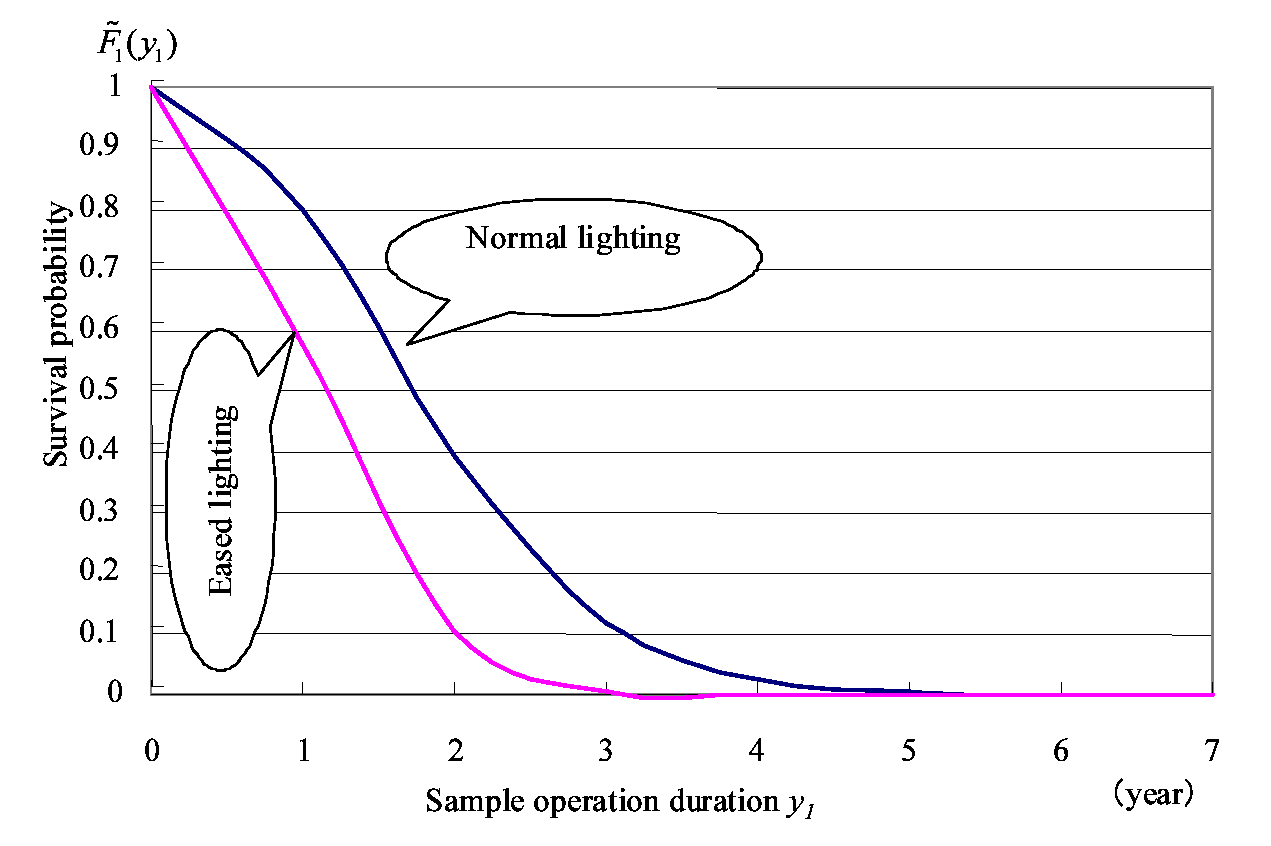
\includegraphics[scale=0.5]{fig32} 
\end{center}
\footnotesize Note) Slopes of survival probabilities $\tilde{F} _ 1(y_1) $ for condition state 1 along operation duration $y_1$ drawn for normal lighting and eased lighting.
\caption{Survival Probability $\tilde{F}_1(y_1)$.}
\label{fig32}
\end{figure}
\begin{figure}[t]
\begin{center}
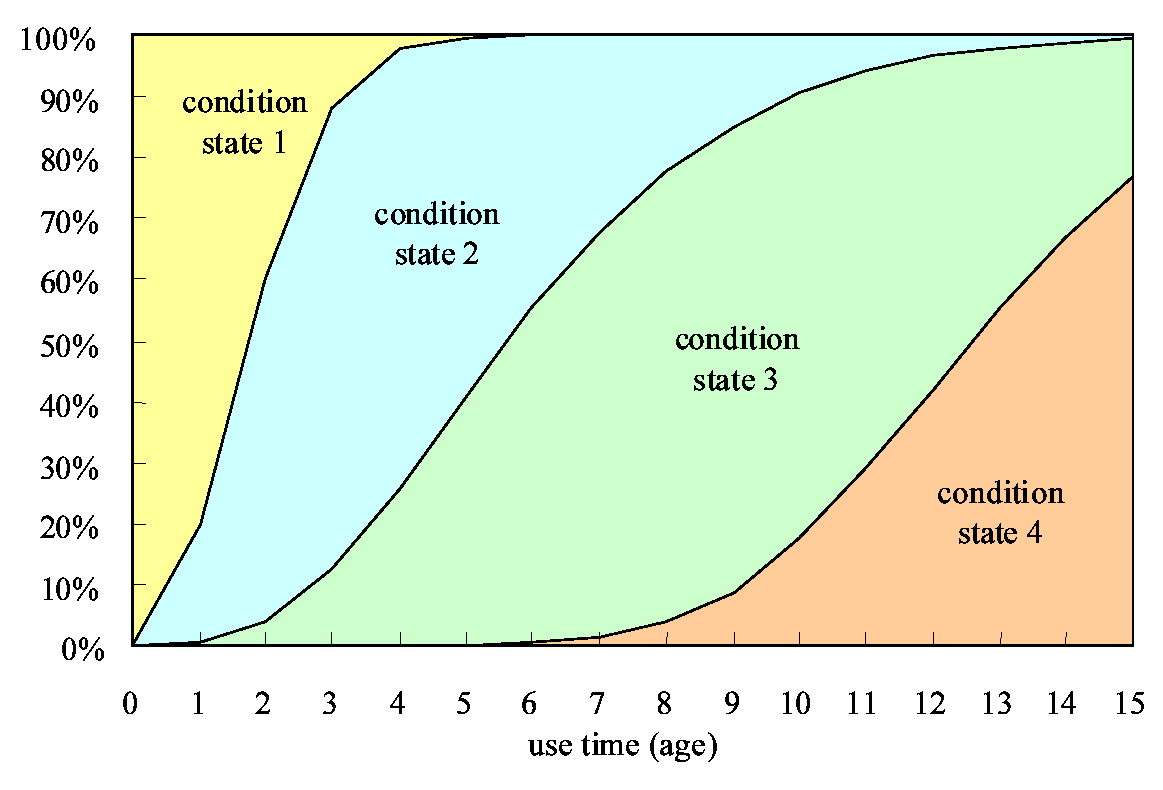
\includegraphics[scale=0.5]{fig33} 
\end{center}
\footnotesize Note) The relation between operation duration $s$ from initial time and deterioration state probability $\pi_i(s) $ for normal lighting.
\caption{Deterioration State Probability $\pi_i(s)$.}
\label{fig33}
\end{figure}
%%
%%
\begin{table}[t]
\begin{center}
\caption{Management Indicator.}
\label{table34}
{\footnotesize
\begin{tabular}{c|c|c|c|c}
 & \multicolumn{2}{|c|}{Life expectancy} & \multicolumn{2}{|c}{Initial life expectancy} \\
Condition state & \multicolumn{2}{|c|}{$RMD(i)$ years} & \multicolumn{2}{|c}{$RL(i)$ years} \\ \cline{2-5}
 & Weibull & Markov & Weibull & Markov \\\hline
1 & 1.45 & 1.23 & 1.45 & 1.27 \\
2 & 4.20 & 3.77 & 5.65 & 5.00 \\
3 & 7.30 & 11.34 & 12.95 & 16.34 \\ \hline
\end{tabular}
}
\end{center}
\footnotesize Note)  Multi-stage Weibull hazard model and multi-stage Markovian hazard model.
\end{table}
%%%
\begin{table}[t]
\begin{center}
\caption{Life Expectancy and Corresponding Condition State $RL_{3}(h(s_A)=i)$.}
\label{table35}
{\footnotesize
\begin{tabular}{c|c|c|c}
Condition state $i$ & $i=1$  & $i=2$ & $i=3$ \\ \hline
$s_A=2$ & 11.85 years & 10.54 years & 6.40 years \\
$s_A=4$ & | & 9.94 years & 5.77 years \\
$s_A=6$ & | & 9.39 years & 4.92 years \\
$s_A=8$ & | & 9.02 years & 3.96 years \\
$s_A=10$ & | & | & 3.15 years \\
$s_A=12$ & | & | & 2.60 years \\ \hline
\end{tabular}
}
\end{center}
\footnotesize Note)  Only elapsed time $s_A$, which displays only the case of survival probability more than 10\%.
\end{table}

Finally, the estimation results for management indicator $RL_{3} (h(s_A)=i) $ are shown in Table \ref{table35}, where values of $RL_{3} (h(s_A)=i) $ are presented  corresponding to the elapsed time $s_A$ and condition state $i$. The values presented in the last column of the table highlights the fact that when elapsed time increases, the life expectancy of condition states tends to decrease.
\section{Summary and Recommendations}
\label{36}
This chapter has presented an analytical methodology using the multi-stage Weibull hazard model for forecasting the deterioration process of infrastructure facilities. The deterioration process is represented by a transition pattern among multiple condition states. In the estimation approach, the maximum likelihood method is employed to estimate the parameters of the model based on observed condition states, characteristic variables and elapsed time of disaggregate samples collected through  inspections.

The proposed model makes it possible to estimate the transition probability of condition states for any arbitrary time intervals. In order to verify the applicability of the model, an empirical study was conducted on a database of tunnel lighting facilities of express highways in Japan. This study has made a contribution to the field by benchmarking findings  with estimation results using the Multi-stage Markovian hazard model. The analytical methodology presented can be extended to apply not only to tunnel lighting facilities but to various other kinds of infrastructure facilities as well.

However, we have not discussed several points, which will be considered as topics for extending this study in the future:
\begin{itemize}
 \item Measurement errors occurring in monitoring and inspection activities have not been addressed in this model. In order to tackle this problem, for example, a methodology using Bayesian estimation and Markov Chain Monte Carlo, for example, can be incorporated into the model in the future.
 \item The samples used in empirical study shared almost similar structural characteristics. However, in general practice, an infrastructure database system is often comprised of heterogeneous groups. Thus, the impacts of individual groups on the overall deterioration process should be investigated. A methodology using the mixture mechanism in hazard analysis can be proposed for future consideration.
 \item In future management, a tendency might develop whereby shorter inspections will become common due to innovations in technology. Hence, the database system of infrastructure management should be designed in such a way that it can be synchronized with an analytical frame. As a sequel, the future focus on multi-schemes inspection data should be considered.
\end{itemize}